\chapter{Implementation}\label{ch:implementation}
\todo{insert code snips, especially the stuff relevant to the database, our architecture, and of course our regression algorithm.}

\section{Regression}
Som nævnt er der i koden brugt regression til at kunne forudsige, hvor mange af hvert produkt, der bliver solgt i fremtiden, så den optimale bestillingsmængde kan beregnes. 
\todo{write about regression}


Til dette bruges en formel for at finde den optimale bestillingsmængde ud fra de data som er tilgængelige. Formlen er bedre kendt som Economic Order Quantity (EOQ) model \cite{EOQ}.

\begin{landscape}
    \begin{figure}[p]
        \centering
        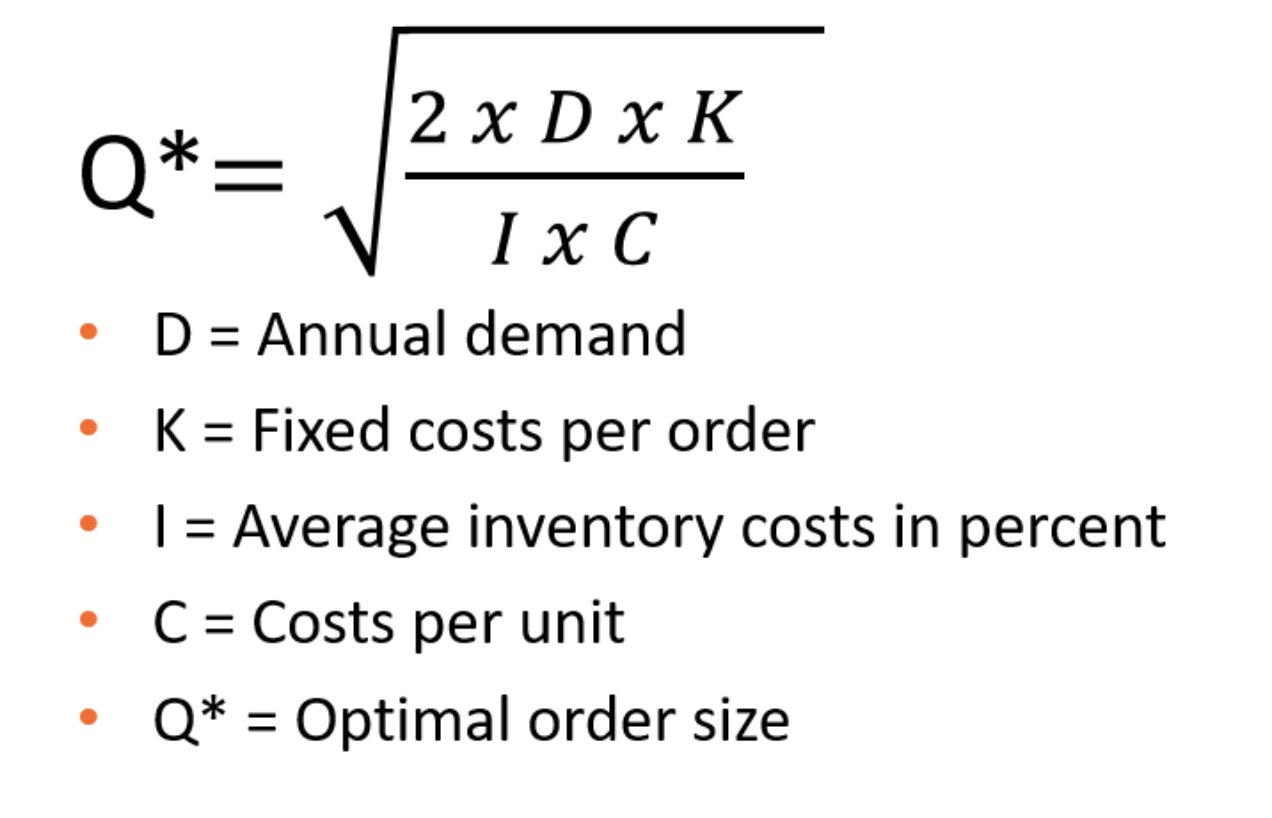
\includegraphics[width=\hsize]{figures/implementation/eoq.png}
        \caption{EOQ formlen - Beregning af den optimale bestillingsmængde}
        \label{fig:eoq}
    \end{figure}
\end{landscape}

Denne formel er så brugt til at beregne samtlige individuelle produkters optimale bestillingsmængde, som så laves til \verb|ProductLine| objekter, som lægges i \verb|PeriodicPlan| så der kan oprettes \verb|StorageOrder|s. 
